\chapter{国内外相关研究现状}\label{chap:related_work}

目前,国内外针对从非结构化文本中进行需求发现和提取已经有一些论文成果。在许多开源和工业项目中,开发人员大量使用书面沟通渠道,例如邮件列表,issue tracker、聊天工具等,并且这样的方式已经遍布全球开发人员的日产工作中。自然语言处理技术和文本挖掘如情感分析、话题建模、机器学习等技术首先被应用于这些文本的意图分类中,如缺陷报告分类、特征请求分类等\cite{maalej2015bug},并且服务于发布计划工具,向应用开发者提供支持,决定哪个新特征需要在下个版本中实现。@@@@@本文主要从@@@@@@几方面介绍国内外相关研究工作。

\section{基于文本数据的需求发现}
如今,软件应用和服务的用户会根据他们的感知体验质量,以简短的评论和排名的形式提供反馈,甚至参与由社交媒体或基于Web的专用交流支持的在线讨论平台,例如App Store,用户论坛,邮件列表,Wiki,新闻组和博客。 这种在线用户反馈的数量迅速增加,代表着软件数据的重要组成部分,并且可以通过软件分析支持软件工程中的决策,从而推动软件工程研究的发展\cite{Morales2019Speech}。 
伴随着这一趋势,在需求工程(RE)中,提出了基于人群的需求工程(CrowdRE)\cite{groen2017crowd}范式,该范式定义了收集,分析和管理人群表达的需求所需的概念,方法和技术集。

人工分析比如基于规则的方法以及有监督的机器学习方法正在大量被应用在分析对软件工程师和非技术利益相关者有用的信息\cite{Morales2019Speech}。
\subsection{基于规则的需求发现}

RE Vlas等人\cite{morales2014discovering}提出一种基于语法的特征请求发现工具。作者使用Subject-action-Object(SAO)语法标签对需求进行解析和表示。其中subject是需求声明的发出者,action定义了需求里面定义的特征,object表示被action影响的对象。比如:“这个提交按钮应该把表单数据提交给处理组件”中,“提交按钮”是subject,“发送”是action,object是“表单数据”。图\ref{fig:sao}是SAO方法对密码安全特征需求进行识别的一个例子。
\begin{figure}[htbp]
    \centering
    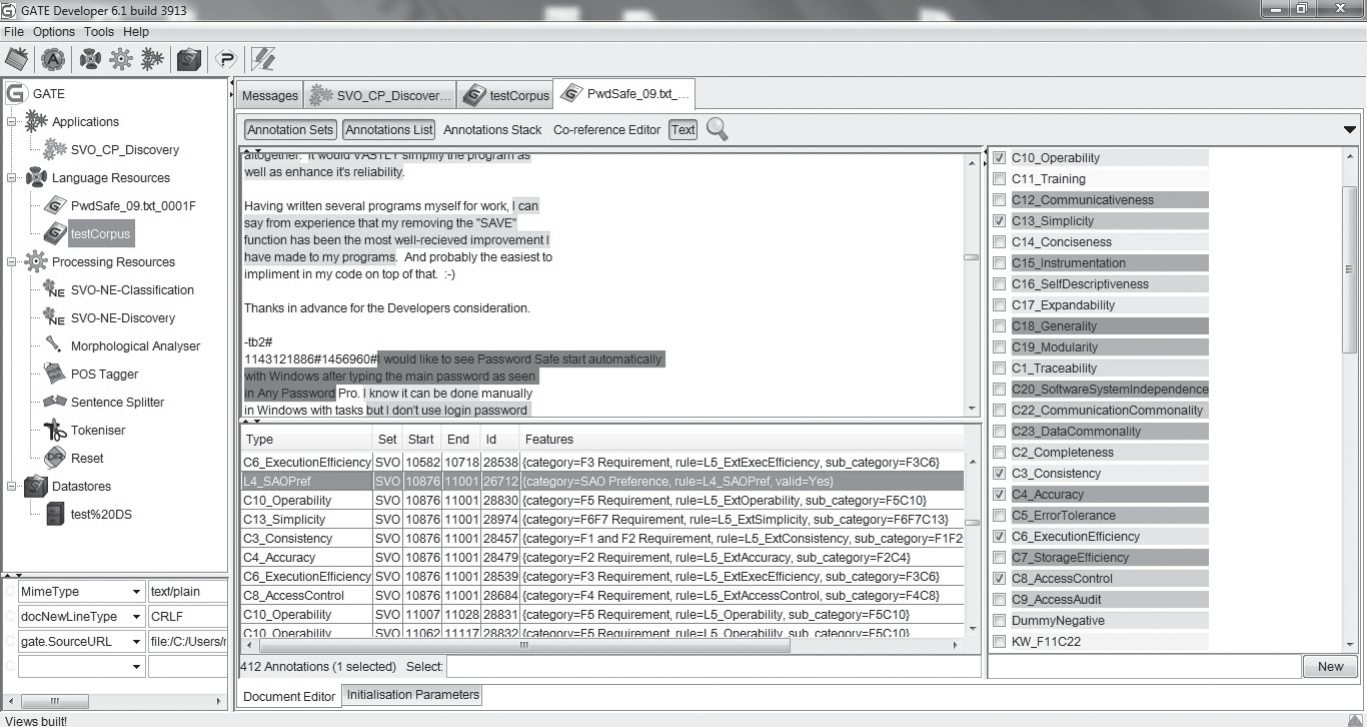
\includegraphics[width=0.70\textwidth]{Img/sao.png}
    \bicaption{基于SAO方法对密码安全特征需求进行识别}{SAO-based Recognized Password Safe Feature Requirements}
    \label{fig:sao}
\end{figure}


邮件是开发者之间进行沟通的重要方式之一,通常包含特征请求、观点询问、问题发现、解决方案、信息提供等不同类别的信息。Di Sorbo等人\cite{Sorbo2016Development}提出一种名叫DECA(开发者电子邮件内容分析器)的半监督学习方法,通过使用自然语言解析工具分析文本的语言学特征并且从询问帮助、提供帮助、提出新需求、报告或者讨论BUG等几方面对开发者的意图进行分类。Di Sorbo等人首先根据来自Ubuntu和QT的数据设置更适合邮件列表信息的分类,具体分类类别如表\ref{tab:deca0}所示。
\begin{table}[htbp]
\bicaption{句子例子以及对应的类别}{Sentence examples and corresponding categories}
    \label{tab:deca0}
    \centering
    \footnotesize% fontsize
    \setlength{\tabcolsep}{4pt}% column separation
    \renewcommand{\arraystretch}{1.2}%row space 
\begin{tabular}{lcccccccc}
\hline
句子类别的例子      & 分类类别 \\
\hline
讨论一个变更       & 特征请求 \\
定位BUG        & 问题发现 \\
BUG是否被修复     & 信息询问 \\
针对已知问题提出解决方案 & 解决方案 \\
请求其他开发者做出变更  & 特征请求 \\
询问代码时如何工作的   & 信息询问 \\
询问为何这样写代码    & 信息询问 \\
向某人征求意见      & 意见询问 \\
找出代码作者       & 信息询问 \\
更多的了解代码      & 信息询问 \\
告诉其他开发者一些事情  & 信息提供 \\
\hline
\end{tabular}
\end{table}
然后对其进行手工标注,作者发现开发人员在关于开发问题的讨论中撰写关于现有错误或者建议提出特征请求时,他们倾向于使用一些经常性的语言模式,比如对于“我们可以使用漏桶算法来限制带宽”,可以发现句子中提供一个明确定义的谓词-参数结构,对此,可以看出大多数具有谓词-论元结构的句子表明解决方案。作者定义了启发式规则,首先发现句子的特定句法结构,然后推广某些类型的信息,最后忽略无用的信息。所以,作者定义了“【某人】可以使用【某事物】”的一般模式来识别解决方案。图\ref{fig:deca1}是作者通过斯坦福依存句法分析来分析启发式规则时的例子。
\begin{figure}[htbp]
    \centering
    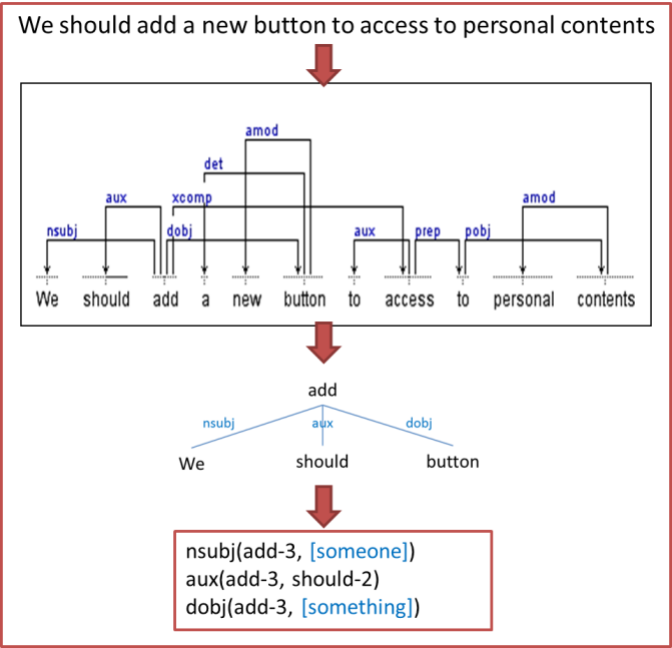
\includegraphics[width=0.70\textwidth]{deca1}
    \bicaption{特征请求中的自然语言解析树}{Natural language parsing tree about feature request}
    \label{fig:deca1}
\end{figure}
作者通过图\ref{fig:deca1}定义了“【某人】应添加【某事物】”的启发规则并于特征请求相关联。Andrea Di Sorbo等人的观点是在软件工程领域始背相关的重复语言模式,这对软件过程中的需求分析非常有用。

L Shi等人\cite{shi2017understanding}提出利用自然语言处理技术生成一组模糊规则来自动分析和构造特征请求的方法,将特征请求中的每个句子进行分类,类别有意图、解释、益处、缺点、示例和无关,分类的结果用来增量生成模糊规则。作者定义了这些类别以及类别的定义和优先级来帮助构建特征请求并突出显示值得关注的内容,如表\ref{tab:fra0}所示。
\begin{table}[htbp]
\bicaption{句子类别的定义}{Definitions of sentence categories}
    \label{tab:fra0}
    \centering
    \footnotesize% fontsize
    \setlength{\tabcolsep}{4pt}% column separation
    \renewcommand{\arraystretch}{1.2}%row space 
\begin{tabular}{lcccccccc}
\hline
类别 & 重要性 & 定义                     \\
\hline
意图 & 1   & 关于改进系统和功能的主意、需求、期望的描述  \\
益处 & 2   & 关于提出的需求带来的好处和有帮助的结果的描述 \\
缺点 & 3   & 关于当前系统行为的缺点            \\
例子 & 4   & 关于支持提出的需求的例子           \\
解释 & 5   & 关于提出需求的场景和解决           \\
无关 & 6   & 和系统无关的信息              \\
\hline
\end{tabular}
\end{table}
作者分别在词汇、语法、语义三个级别启发式地定义模糊规则。词汇通过设置不同类别的词汇表来设置不同句子类别的模式,句法通过对句子进行依存结构分析不同句子类别的句法特征,语义层面通过定义在某个类别的句子中中的语言表达的含义,如图\ref{fig:fra1}所示的语义模式。
\begin{figure}[htbp]
    \centering
    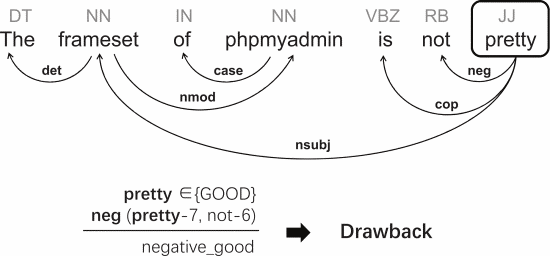
\includegraphics[width=0.70\textwidth]{fra1}
    \bicaption{缺陷类别的语义模式示例}{An example about semantic pattern of defect class}
    \label{fig:fra1}
\end{figure}
实验表明,随着新规则的引入,模糊规则的分类性能越来越高。此外,再将模糊规则转换成布尔变量之后,将其应用于各种机器学习算法上得到了更好的效果。

I Morales-Ramirez等人\cite{Morales2019Speech}关注于分析在线讨论,如开源软件的邮件列表和用户论坛,在这里,不同的利益相关者比如开发者、软件终端用户会讨论有助于软件发展的信息。基于规则Speech-acts分析\cite{morales2014discovering}用在线讨论的自动分析上,比如,通过学生的查询理解学生的意图\cite{feng2006intelligent}等。 Speech-acts理论认为当某人说一些话让对方相信或者做出对应的行为\cite{acts1969essay}。比如在询问一个新特征中使用的词汇包括:“添加特征”、“想要这个特征”等。作者把不同speech-acts规则归为几类:c-Assertive, c-Responsive, c-Requestive和c-Attachment。如表\ref{tab:speech-act0}所示,每一列为对应的独立speech-acts类别。
\begin{table}[htbp]
\bicaption{Speech-acts列表}{List of speech-acts}
    \label{tab:speech-act0}
    \centering
    \footnotesize% fontsize
    \setlength{\tabcolsep}{4pt}% column separation
    \renewcommand{\arraystretch}{1.2}%row space 
\begin{tabular}{lcccccccc}
\hline
c-Assertive & c-Requestive & c-Responsive & c-Attachment & c-Other          \\
\hline
断定        & 请求         & 回应         & 附件         & 描述性的      \\
确认        & 需求         & 建议         & 代码         & 接受           \\
让步        & 问题         & 支持         & URL链接      & 拒绝           \\
            &              &              & 日志文件     & 消极观点 \\
            &              &              &              & 积极观点  \\
            &              &              &              & 感谢            \\
            &              &              &              & 内容丰富的 \\
\hline            
\end{tabular}
\end{table}


基于Speech-acts的模型结构如图\ref{fig:speech-acts1}所示。
\begin{figure}[htbp]
    \centering
    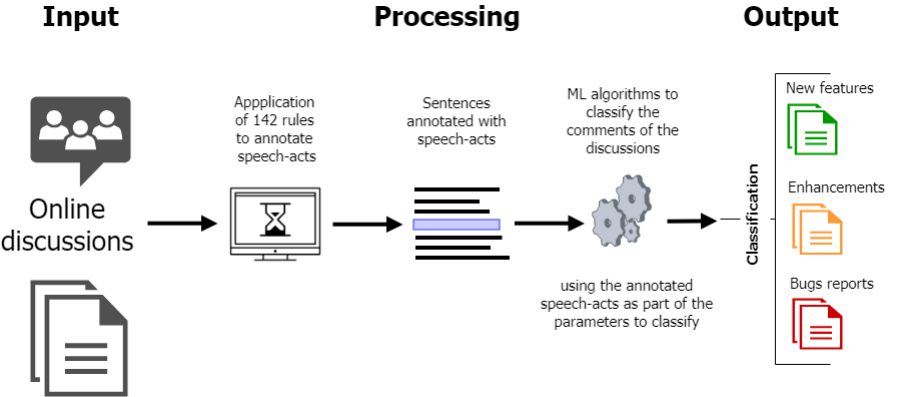
\includegraphics[width=0.70\textwidth]{Img/speech-acts1.png}
    \bicaption{基于Speech-acts的分析模型}{Speech-acts based analysis approach}
    \label{fig:speech-acts1}
\end{figure}
这个工具结合了作者基于他们关于需求的知识以及利益相关者在在线讨论中表达他们需求的方式定义的142条词法-句法规则,从而对特征请求进行发现。

\subsection{基于统计机器学习的需求发现}
开发者和客户通常会通过会面来获取用户故事,P Rodeghero等人\cite{Rodeghero2017Detecting}提出一种从客户和开发人员之间记录的对话中自动提取和用户故事相关的信息。作者从开发人员和客户之间的对话记录中自动提取用于编写用户故事的数据,分别进行定性研究,以检验开发者和客户之间的对话包含用户故事的角色、功能和基本原理的假设,以及定量研究以确定现有分类算法的效果。作者通过定性研究分析得到大约5.5\%的对话包含功能信息,2.9\%包含了基本原理,只有0.5\%讨论了角色,发现对话包含重要的功能和基本原理信息,但关于角色的数据非常有限。作者训练了一个分类器用于检测包含功能数据的对话部分。在数据收集部分,作者收集一家软件开发公司的会议记录,并标注文件名、会话、摘要、会话转折、角色、功能、理由等信息,作者提取了25个属性进行分类,并且分析的单位是转折而不是句子,提出的方法模型如图\ref{fig:Rodeghero2017Detecting}所示。
\begin{figure}[htbp]
    \centering
    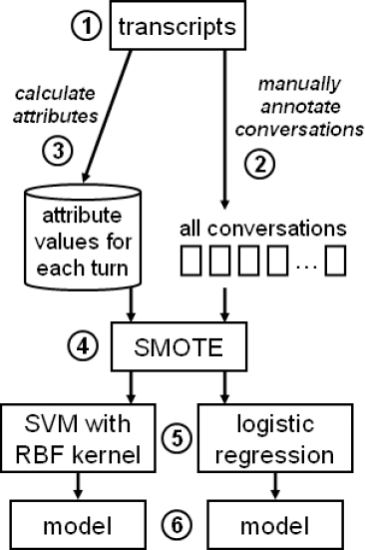
\includegraphics[width=0.40\textwidth]{Rodeghero2017Detecting.png}
    \bicaption{分类器模型结构图}{Structure of classifier}
    \label{fig:Rodeghero2017Detecting}
\end{figure}

Q Huang等人\cite{Huang2018Automating}发现Di Sorbo等人的分类类别还有55\%的句子不能覆盖,于是在其分类的基础上合并了两种意图,并新增了两种意图,提炼过的分类类别如表\ref{tab:aim0}所示。
\begin{table}[htbp]
\bicaption{精炼后的意图分类}{Intention classification after refine}
    \label{tab:aim0}
    \centering
    \footnotesize% fontsize
    \setlength{\tabcolsep}{4pt}% column separation
    \renewcommand{\arraystretch}{1.2}%row space 
\begin{tabular}{lcccccccc}
\hline
类别   & 描述                 \\
\hline
信息提供 & 将知识、经验、计划、更新共享给其他人 \\
信息寻找 & 希望得到信息和帮助          \\
特征请求 & 帮助改进现有功能或提出新功能     \\
解决方案 & 共享可能的解决方案          \\
问题发现 & 报告BUG,或描述异常行为      \\
侧面评价 & 表达观点或进行评价          \\
无意义  & 无意义的或不重要的         \\
\hline
\end{tabular}
\end{table}
并提出了使用Convolutional Neural Network(CNN)\cite{kim2014convolutional}的方法自动将句子分类为不同的意图类别,整体模型架构如图\ref{fig:aim1}所示。
\begin{figure}[htbp]
    \centering
    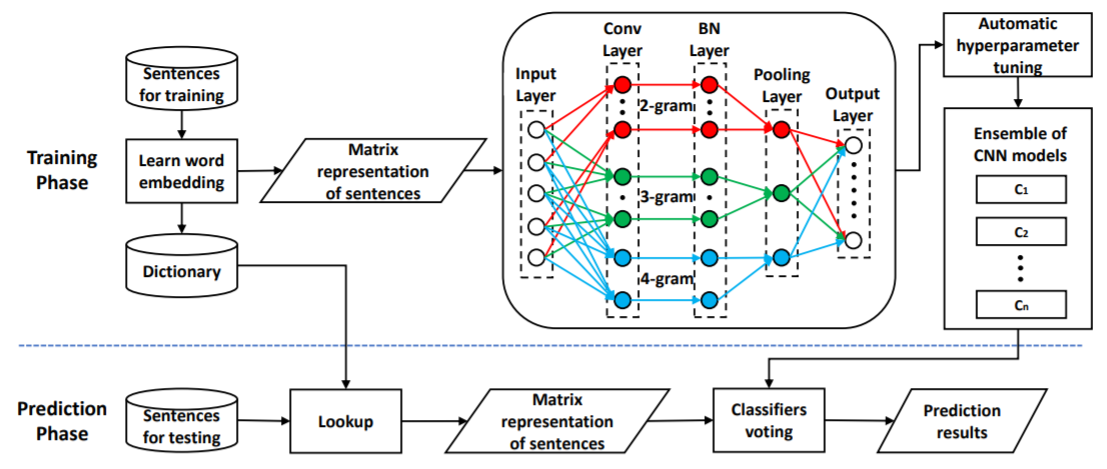
\includegraphics[width=\textwidth]{aim1.png}
    \bicaption{CNN分类模型整体框架}{Structure of CNN classifier}
    \label{fig:aim1}
\end{figure}
CNN将句子作为输入,输入7个概率值,从而得出概率最大的句子类别,即使测试集中没有出现和训练集相似的模式或者关键词,模型也会给出概率最大的类别,从而覆盖所有句子。

Y Zhang等人\cite{zhang2015sensitivity}发现词向量的维度、过滤器的数量以及过滤器的深度是影响较大的超参数,作者使用贪婪的方式搜索最优参数。
D Arya等人\cite{arya2019analysis}通过对15个问题讨论进行内容定量分析确定包括潜在特征请求在内的16种信息类型。作者手工构建了14个对话特征,并使用随机森林作为分类器,对表达新特征请求的句子可以达到66\%的F1值。
W Maalej等人\cite{maalej2015bug}使用自然语言处理技术包括文本分类、情感分析把App Reviews分类为缺陷报告、特征请求、用户经验和打分。其中分类结果的precision可达到70-95\%,recall可达到80-90\%。
\section{聊天对话文本在软件工程中的应用}
在各种软件开发项目中,两种常见的聊天方式为同步和异步沟通方式\cite{yu2011communications}。同步方式包括Internet Relay Chat(IRC)等聊天工具,异步方式包括邮件列表、Issue tracker等工具。
基于Web平台的关于软件应用和服务的在线聊天讨论在包括需求发现等各种软件工程任务中表现出来巨大的价值\cite{Morales2019Speech},目前已有大量的研究工作正在开发有效的工具支持软件分析。它们利用自然语言处理技术从应用商店评论、在线聊天记录、邮件列表、用户论坛等文本数据中抽取相关信息,并且使用文本挖掘和机器学习技术对信息进行分类如缺陷报告或者特征请求。其中聊天记录中包含着关于软件系统的丰富的信息。

B Lin等人\cite{lin2016developers}通过一项关于开发者怎么使用Slack、哪个聊天工具在开源社区比较流行、聊天工具能够为软件开发带来怎么样的好处的研究,发现开发者使用Slack进行个人、团队、社区级别的交流,Slack也占据越来越重要的地位,在某些情况下会代替邮件。
E Shihab等人\cite{shihab2009studying}通过两个大型开源项目从几个维度分析了开发者IRC会议:会议内容、会议参与者、他们的贡献、会议类型。作者的研究表明IRC正在开源社区占据越来越重要的地位,强调了从开发者聊天记录中可以获取丰富的信息。
P Chatterjee等人\cite{chatterjee2019exploratory}调查了通过挖掘开发者谈话从而支持软件维护和演化的有效性和挑战性,作者发现开发者倾向于通过即时聊天工具分享对于观点或者有意义的想法,并且说明了通过应用一些技术和训练集可以达到较高的对话解耦效果。

\section{自然语言处理中的对话解耦}
\subsection{对话解耦}


\section{自然语言文本的嵌入式表示和文本分类}
\subsection{TF-IDF}
\subsection{文本嵌入式表达}
\subsection{Convolutional Neural Network}
\subsection{Long Sequence Term Machine}
\subsection{文本分类模型}

\section{少样本学习}


